% ======== 卷一（8行21字）========
\chapter*{欽定儀象考成卷一}
\begin{正文}
\end{正文}\clearpage
\thispagestyle{empty}\noindent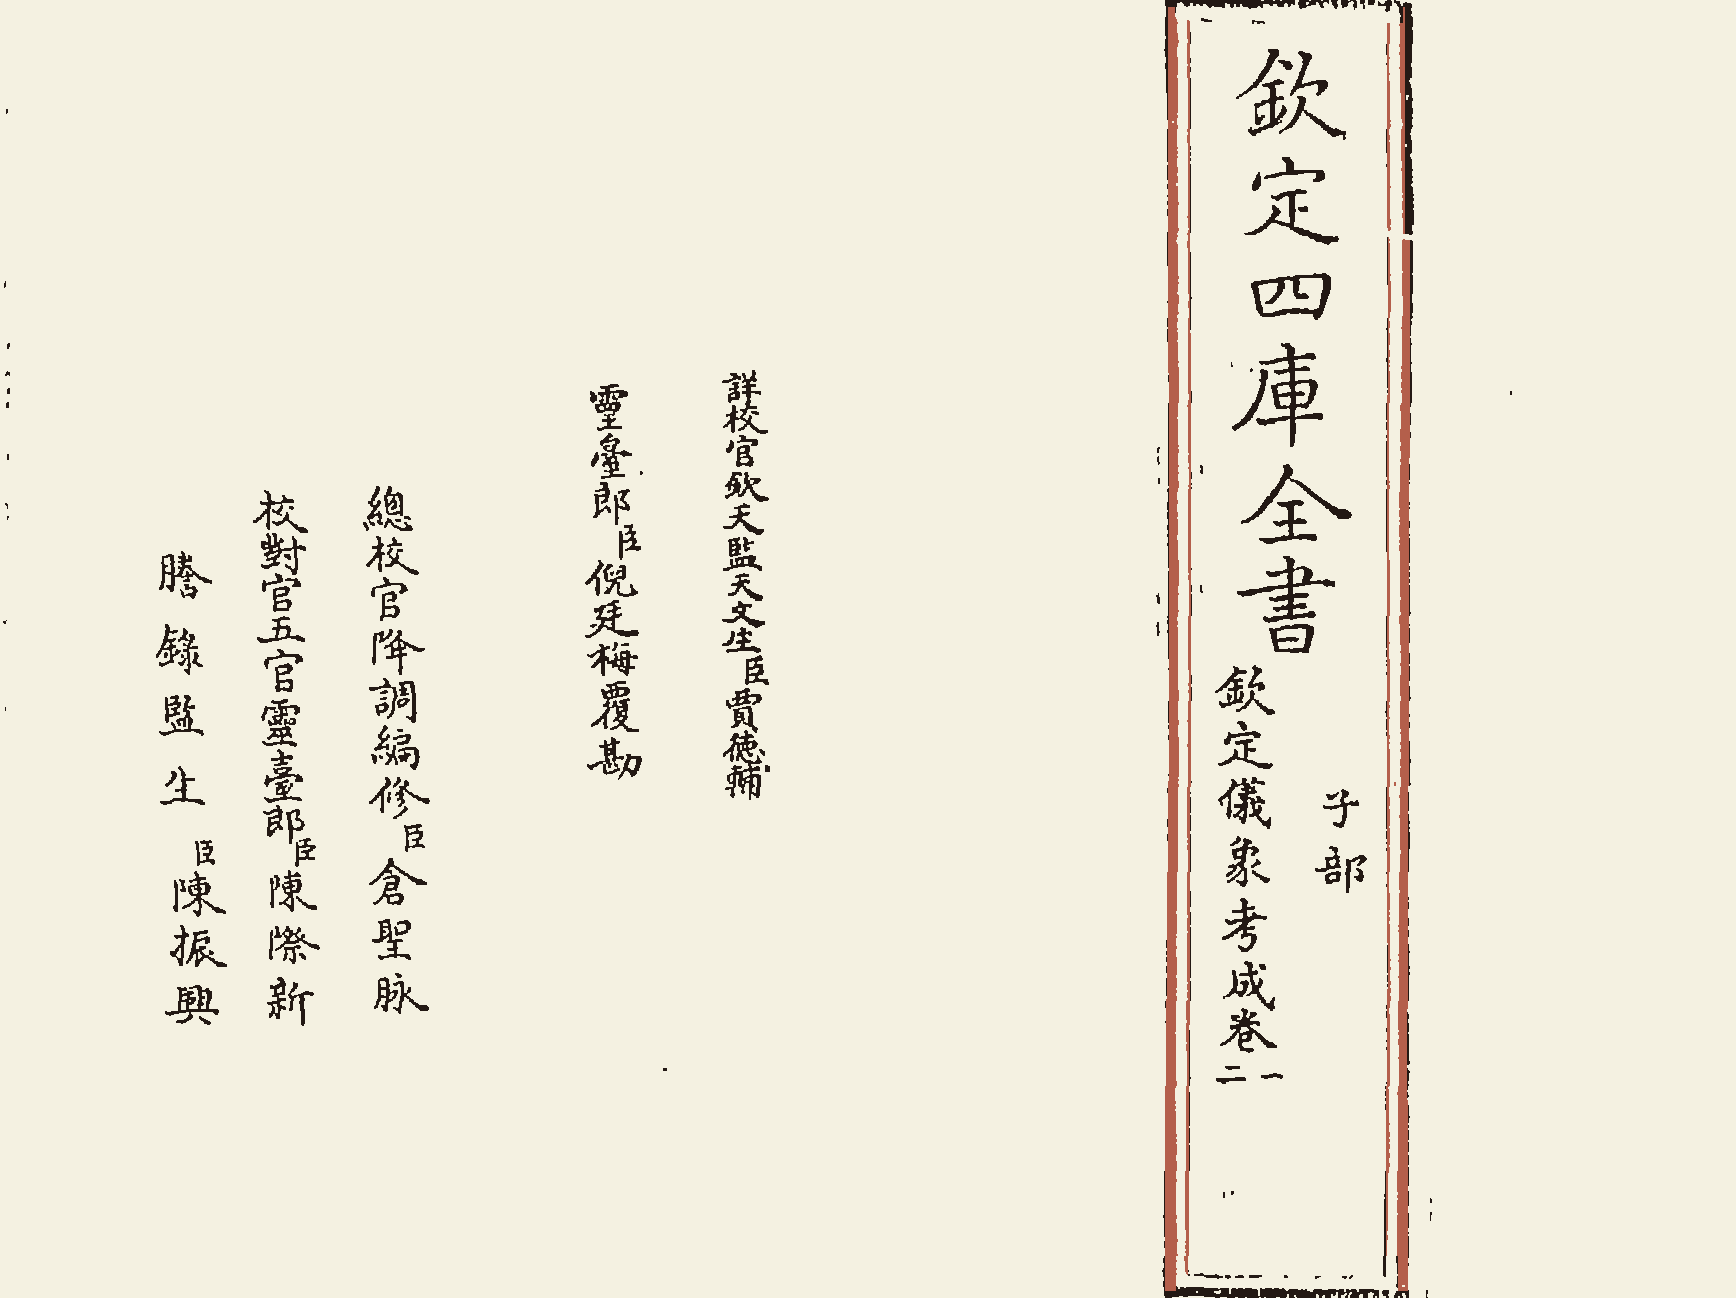
\includegraphics[width=\paperwidth,height=\paperheight,keepaspectratio]{img/0400.png}\clearpage
\begin{正文}
% ---- 册793 葉401 ----
\SetPageNumber{1}
欽定四庫全書\换行
欽定儀象考成卷一\换行
　恒星總紀\换行
　　三垣\换行
　　一十八宿\换行
　　恒星全圖\换行
　　赤道北恒星圖\换行
　　赤道南恒星圖\换行
\char"200B\relax\换行
\char"200B\relax\换行
\char"200B\relax\换行
\char"200B\relax\换行
\char"200B\relax\换行
\char"200B\relax\换行
\char"200B\relax\换行
\char"200B\relax
\par
% ---- 册793 葉404 ----
　　恒星總紀\换行
恒星即經星也以其有常不易故名經星\双列{\右小列{史記天官書}\左小列{紫宫房心權}}\换行
\双列{\右小列{衡咸池虚危列宿部星此天之五宫坐}\左小列{位也為經不移徙大小有差濶狹有常}}經星又各有經\换行
緯度故别之曰恒星其星官名數古今不同漢書天文\换行
志經星常宿中外官凡百一十八名積數七百八十三\换行
星晉志載呉太史令陳卓始列甘石巫咸三家星官著\换行
於圖録凡二百八十三官一千四百六十四星今皆不\换行
見原本隋丹元子歩天歌與陳卓數合後此言天官者\换行
皆以歩天歌為凖康熙十三年監臣南懐仁修儀象志\换行
星名與古同者總二百五十九座一千一百二十九星\换行
比歩天歌少二十四座三百三十五星又於有名常數\换行
之外増五百九十七星又多近南極星二十三座一百\换行
五十星近年以來累加測騐星官度數儀象志尚多未\换行
合又星之次第多不順序亦宜釐正於是逐星測量推\换行
其度數觀其形象序其次第著之於圖計三垣二十八\换行
宿星名與古同者總二百七十七座一千三百一十九
\par
% ---- 册793 葉405 ----
星比儀象志多十八座一百九十星與歩天歌為近其\换行
尤與古合者二十八宿次舍自古皆觜宿在前參宿在\换行
後其以何星作距古無明文唐書云古以參右肩為距\换行
失之太逺文獻通考載宋兩朝天文志云觜三星距西\换行
南星參十星距中星西第一星西法觜宿距中上星參\换行
宿亦距中西一星今按觜宿中上星在西南星前僅六\换行
分餘而西南星小中上星大則以中上星作距可也若\换行
參宿以中西一星作距星則觜宿之黄道度已在參宿\换行
後一度餘即赤道度亦在參宿後三十一分餘今依次\换行
順序以參宿中三星之東一星作距星則觜宿黄道度\换行
恒在參前一度弱與觜前參後之序合其餘諸座之星\换行
皆以次順序無凌躐顛倒之弊又於有名常數之外増\换行
一千六百一十四星近某座者即名某座増星依次分\换行
註方位以備稽考其近南極星二十三座一百五十星\换行
中國所不見仍依西測之舊共計恒星三百座三千八\换行
十三星編為總紀一卷庶星官名數古今不同及黄道
\par
% ---- 册793 葉408 ----
赤道所屬宫次皆展卷瞭然矣\换行
\char"200B\relax\换行
\char"200B\relax\换行
\char"200B\relax\换行
\char"200B\relax\换行
\char"200B\relax\换行
\char"200B\relax\换行
\char"200B\relax\换行
\char"200B\relax\换行
\char"200B\relax\换行
\char"200B\relax\换行
\char"200B\relax\换行
\char"200B\relax\换行
\char"200B\relax\换行
\char"200B\relax\换行
\char"200B\relax
\par
% ---- 册793 葉409 ----
紫微垣\换行
北極五星一太子二帝星三庶子四后宫五天樞外庶\换行
子増三星后宫増一星黄道在午未宫赤道在卯辰宫\换行
四輔四星外増一星黄道在未宫赤道在已午宫\换行
勾陳六星外増十星黄道在未申宫赤道在丑寅卯戌\换行
亥宫\换行
天皇大帝一星黄道在申宫赤道在亥宫\换行
天柱五星外増六星黄道在申酉宫赤道在子丑宫\换行
御女四星外増一星黄道在未申酉宫赤道在丑寅宫\换行
女史一星外増一星黄道在未宫赤道在寅宫\换行
柱史一星外増二星黄道在申宫赤道在丑宫\换行
尚書五星外増二星黄道在辰已午宫赤道在寅宫\换行
天床六星外増一星黄道在巳午宫赤道在寅卯宫\换行
大理二星外増一星黄道在未宫赤道在辰巳宫\换行
陰德二星外増一星黄道在未宫赤道在巳宫\换行
六甲六星外増一星黄道赤道俱在未申宫
\par
% ---- 册793 葉412 ----
五帝内座五星外増二星黄道在申宫赤道在酉戌宫\换行
華葢七星黄道在酉宫赤道在戌宫\换行
杠九星附華葢為一座外増一星黄道在申酉宫赤道\换行
在酉戌宫\换行
右垣墻七星一右樞二少尉三上輔四少輔五上衛六\换行
少衛七上丞外少尉増二星上輔増二星少輔増一星\换行
上衛増三星少衛増一星上丞増三星黄道在已午未\换行
申宫赤道在辰已午未申酉宫\换行
左垣墻八星一左樞二上宰三少宰四上弼五少弼六\换行
上衛七少衛八少丞外上衛増三星少衛増八星少丞\换行
増一星黄道在辰已酉宫赤道在戌亥子丑寅卯宫\换行
天乙一星黄道在已宫赤道在辰宫\换行
太乙一星黄道在午宫赤道在辰宫\换行
内厨二星外増二星黄道在午宫赤道在辰宫\换行
北斗七星一天樞二天璇三天璣四天權五玉衡六開\换行
陽七揺光外天樞増三星天璇増八星天權増三星開
\par
% ---- 册793 葉413 ----
陽増二星黄道在已午宫赤道在辰已宫\换行
輔一星附北斗為一座外増三星黄道在已宫赤道在\换行
辰宫\换行
天槍三星外増四星黄道在已宫赤道在卯宫\换行
元戈一星外増二星黄道在辰宫赤道在卯宫\换行
三公三星黄道在已宫赤道在辰宫\换行
相一星外増三星黄道在已宫赤道在辰宫\换行
天理四星外増一星黄道在午宫赤道在已宫\换行
太陽守一星外増一星黄道赤道俱在巳宫\换行
太尊一星黄道在午宫赤道在巳宫\换行
天牢六星外増二星黄道在巳午宫赤道在巳宫\换行
勢四星外増十六星黄道在午宫赤道在巳宫\换行
文昌六星外増八星黄道在午未宫赤道在午宫\换行
内階六星外増十星黄道在未宫赤道在午宫\换行
三師三星外増一星黄道在未宫赤道在午宫\换行
八榖八星外増三十四星黄道赤道俱在申宫
\par
% ---- 册793 葉416 ----
傳舍九星外増四星黄道在申酉宫赤道在酉戌亥宫\换行
天厨六星外増二星黄道在戌宫赤道在子丑宫\换行
天棓五星外増十星黄道赤道俱在寅宫\换行
　右共三十七座一百六十三星外増一百七十七星\换行
太微垣\换行
五帝座五星外増三星黄道赤道俱在巳宫\换行
太子一星黄道赤道俱在巳宫\换行
從官一星黄道赤道俱在巳宫\换行
幸臣一星黄道赤道俱在巳宫\换行
五諸侯五星外増七星黄道在辰巳宫赤道在辰宫\换行
九卿三星外増九星黄道赤道俱在辰宫\换行
三公三星黄道赤道俱在辰宫\换行
内屏四星外増六星黄道赤道俱在巳宫\换行
右垣墻五星一右執法二上將三次將四次相五上相\换行
外次相増三星上相増二星黄道赤道俱在巳宫\换行
左垣墻五星一左執法二上相三次相四次將五上將
\par
% ---- 册793 葉417 ----
外左執法增一星次相増一星次將増三星上將増二\换行
星黄道赤道俱在辰宫\换行
郎將一星外増二星黄道在巳宫赤道在辰宫\换行
郎位十五星外増三星黄道在巳宫赤道在辰巳宫\换行
常陳七星外増六星黄道在巳宫赤道在辰巳宫\换行
三台六星上台二星中台二星下台二星外上台増七\换行
星中台増三星下台増二星黄道在巳午未宫赤道在\换行
巳午宫\换行
虎賁一星黄道赤道俱在巳宫\换行
少微四星外增八星黄道在巳午宫赤道在巳宫\换行
長垣四星外増九星黄道在巳午宫赤道在巳宫\换行
靈臺三星外増八星黄道赤道俱在巳宫\换行
明堂三星外増六星黄道赤道俱在巳宫\换行
謁者一星外増二星黄道在巳宫赤道在辰宫\换行
　右共二十座七十八星外増九十三星\换行
天市垣
\par
% ---- 册793 葉420 ----
帝座一星黄道赤道俱在寅宫\换行
候一星外増五星黄道赤道俱在寅宫\换行
宦者四星外増五星黄道赤道俱在寅宫\换行
斗五星外増十四星黄道在寅卯宫赤道在寅宫\换行
斛四星外増三星黄道赤道俱在寅宫\换行
列肆二星外増四星黄道在寅卯宫赤道在寅宫\换行
車肆二星外増二星黄道赤道俱在寅宫\换行
市樓六星外増一星黄道赤道俱在寅宫\换行
宗正二星外増三星黄道赤道俱在寅宫\换行
宗人四星外増四星黄道赤道俱在寅宫\换行
宗二星黄道赤道俱在丑宫\换行
帛度二星外増三星黄道赤道俱在寅宫\换行
屠肆二星外増三星黄道赤道俱在丑寅宫\换行
右垣墻十一星一河中二河間三晉四鄭五周六秦七\换行
蜀八巴九梁十楚十一韓外河間増一星晉増三星周\换行
増十四星秦増一星蜀増二星巴増四星黄道赤道俱
\par
% ---- 册793 葉421 ----
在寅卯宫\换行
左垣墻十一星一魏二趙三九河四中山五齊六呉越\换行
七徐八東海九燕十南海十一宋外魏増八星趙増三\换行
星九河増一星中山増七星齊増八星呉越増七星徐\换行
増四星東海増四星宋増二星黄道赤道俱在丑寅宫\换行
天紀九星外増十四星黄道在寅卯宫赤道在寅宫\换行
女牀三星黄道赤道俱在寅宫\换行
貫索九星外増十三星黄道赤道俱在卯宫\换行
七公七星外増十六星黄道在卯辰宫赤道在寅卯宫\换行
　右共十九座八十七星外増一百五十九星\换行
角宿\换行
角宿二星外増十五星黄道赤道俱在辰宫\换行
平道二星黄道赤道俱在辰宫\换行
天田二星外増六星黄道赤道俱在辰宫\换行
周鼎三星黄道在辰巳宫赤道在辰宫\换行
進賢一星外増九星黄道赤道俱在辰宫
\par
% ---- 册793 葉424 ----
天門二星外増十一星黄道赤道俱在辰宫\换行
平二星外増三星黄道在卯辰宫赤道在辰宫\换行
庫樓十星外増一星黄道赤道俱在卯辰宫\换行
柱十一星黄道赤道俱在卯辰宫\换行
衡四星黄道在卯宫赤道在辰宫\换行
南門二星外増二星黄道在卯宫赤道在卯辰宫\换行
　右共十一座四十一星外増四十七星\换行
亢宿\换行
亢宿四星外増十二星黄道在卯宫赤道在卯辰宫\换行
大角一星外増一星黄道在辰宫赤道在卯宫\换行
右攝提三星外増三星黄道赤道俱在辰宫\换行
左攝提三星外増三星黄道在卯辰宫赤道在卯宫\换行
折威七星外増六星黄道赤道俱在卯宫\换行
頓頑二星外増一星黄道赤道俱在卯宫\换行
陽門二星黄道赤道俱在卯宫\换行
　右共七座二十二星外増二十六星
\par
% ---- 册793 葉425 ----
氐宿\换行
氐宿四星外増二十九星黄道赤道俱在卯宫\换行
亢池四星黄道在辰宫赤道在卯辰宫\换行
帝席三星外増一星黄道赤道俱在辰宫\换行
梗河三星外増五星黄道在卯辰宫赤道在卯宫\换行
招揺一星黄道在辰宫赤道在卯宫\换行
天乳一星外増三星黄道赤道俱在卯宫\换行
天輻二星外増一星黄道赤道俱在卯宫\换行
陣車三星外増二星黄道赤道俱在卯宫\换行
騎官十星黄道赤道俱在卯宫\换行
車騎三星黄道赤道俱在卯宫\换行
將軍一星黄道赤道俱在卯宫\换行
　右共十一座三十五星外増四十一星\换行
房宿\换行
房宿四星外増六星黄道赤道俱在卯宫\换行
鈎鈐二星附房宿為一座黄道在寅宫赤道在卯宫
\par
% ---- 册793 葉428 ----
鍵閉一星黄道在卯宫赤道在寅宫\换行
罰三星外増三星黄道在卯宫赤道在寅卯宫\换行
西咸四星外増二星黄道赤道俱在卯宫\换行
東咸四星外増一星黄道赤道俱在寅宫\换行
日一星外増一星黄道赤道俱在卯宫\换行
從官二星外増一星黄道赤道俱在卯宫\换行
　右共七座二十一星外増十四星\换行
心宿\换行
心宿三星外増八星黄道赤道俱在寅宫\换行
積卒二星黄道在寅宫赤道在卯宫\换行
　右共二座五星外増八星\换行
尾宿\换行
尾宿九星外増一星黄道赤道俱在寅宫\换行
神宫一星附尾宿為一座黄道赤道俱在寅宫\换行
天江四星外増十一星黄道赤道俱在寅宫\换行
傅説一星黄道赤道俱在寅宫
\par
% ---- 册793 葉429 ----
魚一星黄道赤道俱在寅宫\换行
龜五星黄道赤道俱在寅宫\换行
　右共五座二十一星外増十二星\换行
箕宿\换行
箕宿四星黄道赤道俱在丑寅宫\换行
糠一星黄道赤道俱在寅宫\换行
杵三星外増一星黄道赤道俱在寅宫\换行
　右共三座八星外増一星\换行
斗宿\换行
斗宿六星外増四星黄道赤道俱在丑寅宫\换行
天籥八星外増四星黄道赤道俱在寅宫\换行
天弁九星外増五星黄道赤道俱在丑宫\换行
建六星外増八星黄道赤道俱在丑宫\换行
天雞二星外増三星黄道赤道俱在丑宫\换行
狗二星外増六星黄道赤道俱在丑宫\换行
狗國四星黄道赤道俱在丑宫
\par
% ---- 册793 葉432 ----
天淵三星黄道赤道俱在丑宫\换行
農丈人一星黄道赤道俱在丑宫\换行
鼈十一星黄道赤道俱在丑宫\换行
　右共十座五十二星外増三十星\换行
牛宿\换行
牛宿六星外増九星黄道赤道俱在子丑宫\换行
天桴四星外増二星黄道在子丑宫赤道在丑宫\换行
河鼓三星外増九星黄道赤道俱在丑宫\换行
右旗九星外増十二星黄道赤道俱在丑宫\换行
左旗九星外増二十九星黄道赤道俱在子丑宫\换行
織女三星外増四星黄道赤道俱在丑宫\换行
漸臺四星外増六星黄道赤道俱在丑宫\换行
輦道五星外増九星黄道在子丑宫赤道在丑宫\换行
羅堰三星外增一星黄道赤道俱在子宫\换行
天田四星黄道赤道俱在子宫\换行
九坎四星黄道赤道俱在子宫
\par
% ---- 册793 葉433 ----
　右共十一座五十四星外増八十一星\换行
女宿\换行
女宿四星外増五星黄道赤道俱在子宫\换行
離珠四星外増一星黄道赤道俱在子宫\换行
敗𤓰五星外増三星黄道赤道俱在子宫\换行
瓠𤓰五星外増五星黄道赤道俱在子宫\换行
天津九星外増三十八星黄道在亥子宫赤道在子丑\换行
宫\换行
奚仲四星外増七星黄道在子宫赤道在丑宫\换行
扶筐七星外増四星黄道在子丑宫赤道在丑宫\换行
十二國十六星周二星秦二星代二星趙二星越一星\换行
齊一星楚一星鄭一星魏一星韓一星晉一星燕一星\换行
外代増二星黄道赤道俱在子宫\换行
　右共八座五十四星外増六十五星\换行
虚宿\换行
虚宿二星外増八星黄道赤道俱在子宫
\par
% ---- 册793 葉436 ----
司命二星黄道赤道俱在子宫\换行
司禄二星外増二星黄道赤道俱在子宫\换行
司危二星黄道赤道俱在子宫\换行
司非二星外増二星黄道赤道俱在子宫\换行
哭二星外増四星黄道赤道俱在子宫\换行
泣二星外増二星黄道在亥子宫赤道在亥宫\换行
離瑜三星外増三星黄道赤道俱在子宫\换行
天壘城十三星黄道赤道俱在子宫\换行
敗臼四星外増一星黄道在子宫赤道在亥子宫\换行
　右共十座三十四星外増二十二星\换行
危宿\换行
危宿三星外増十一星黄道在亥子宫赤道在子宫\换行
墳墓四星附危宿為一座外増四星黄道赤道俱在亥\换行
宫\换行
葢屋二星黄道赤道俱在子宫\换行
虚梁四星黄道赤道俱在亥宫
\par
% ---- 册793 葉437 ----
天錢五星外増四星黄道赤道俱在子宫\换行
人四星外増四星黄道在亥子宫赤道在子宫\换行
杵三星外増二星黄道在亥宫赤道在亥子宫\换行
臼四星外増五星黄道在亥宫赤道在亥子宫\换行
車府七星外増十九星黄道在戌亥宫赤道在亥子宫\换行
造父五星外増五星黄道在戌宫赤道在亥子宫\换行
天鉤九星外増十六星黄道在酉戌宫赤道在亥子宫\换行
　右共十座五十星外増七十星\换行
室宿\换行
室宿二星外増七星黄道赤道俱在亥宫\换行
離宫六星附室宿為一座外増八星黄道赤道俱在亥\换行
宫\换行
螣蛇二十二星外増十四星黄道在戌亥宫赤道在亥\换行
子宫\换行
雷電六星外増八星黄道赤道俱在亥宫\换行
土公吏二星黄道赤道俱在亥宫
\par
% ---- 册793 葉440 ----
壘壁陣十二星外増七星黄道赤道俱在亥子宫\换行
羽林軍四十五星黄道赤道俱在亥子宫\换行
天綱一星黄道在子宫赤道在亥宫\换行
北落師門一星黄道赤道俱在亥宫\换行
鈇鉞三星外増二星黄道赤道俱在亥宫\换行
八魁六星黄道在亥宫赤道在戌亥宫\换行
　右共十座一百零六星外増四十六星\换行
壁宿\换行
壁宿二星外増二十三星黄道在戌宫赤道在戌亥宫\换行
天廐三星外増一星黄道赤道俱在戌宫\换行
土公二星外増十一星黄道在戌宫赤道在戌亥宫\换行
霹𩆝五星外増八星黄道赤道俱在亥宫\换行
雲雨四星外増九星黄道赤道俱在亥宫\换行
鈇鑕五星黄道赤道俱在戌宫\换行
　右共六座二十一星外増五十二星\换行
奎宿
\par
% ---- 册793 葉441 ----
奎宿十六星外増二十二星黄道赤道俱在戌宫\换行
王良五星外増五星黄道在酉宫赤道在戌亥宫\换行
䇿一星黄道在酉宫赤道在戌宫\换行
附路一星黄道在酉宫赤道在戌宫\换行
軍南門一星黄道在酉宫赤道在戌宫\换行
閣道六星外増五星黄道赤道俱在酉戌宫\换行
外屏七星外増十五星黄道赤道俱在戌宫\换行
天溷四星外増六星黄道赤道俱在戌宫\换行
土司空一星黄道在亥宫赤道在戌宫\换行
　右共九座四十二星外増五十三星\换行
婁宿\换行
婁宿三星外増十五星黄道在酉戌宫赤道在戌宫\换行
天大將軍十一星外増十六星黄道在酉宫赤道在酉\换行
戌宫\换行
右更五星外増五星黄道赤道俱在戌宫\换行
左更五星外増七星黄道赤道俱在酉宫
\par
% ---- 册793 葉444 ----
天倉六星外増十八星黄道在戌亥宫赤道在戌宫\换行
天庾三星外増三星黄道在戌宫赤道在酉戌宫\换行
　右共六座三十三星外増六十四星\换行
胃宿\换行
胃宿三星外増五星黄道赤道俱在酉宫\换行
大陵八星外増二十星黄道赤道俱在酉宫\换行
積尸一星黄道赤道俱在酉宫\换行
天船九星外増九星黄道在申酉宫赤道在酉宫\换行
積水一星外増一星黄道在申宫赤道在酉宫\换行
天廩四星外増二星黄道赤道俱在酉宫\换行
天囷十三星外増二十星黄道赤道俱在酉戌宫\换行
　右共七座三十九星外増五十七星\换行
昴宿\换行
昴宿七星外増五星黄道赤道俱在酉宫\换行
天阿一星黄道赤道俱在酉宫\换行
月一星外増一星黄道赤道俱在酉宫
\par
% ---- 册793 葉445 ----
卷舌六星外増六星黄道在申酉宫赤道在酉宫\换行
天讒一星黄道赤道俱在酉宫\换行
礪石四星黄道在申宫赤道在申酉宫\换行
天陰五星外増四星黄道赤道俱在酉宫\换行
蒭藁六星外増五星黄道在戌宫赤道在酉宫\换行
天苑十六星外増十六星黄道在酉戌宫赤道在酉宫\换行
　右共九座四十七星外増三十七星\换行
畢宿\换行
畢宿八星外増十三星黄道赤道俱在申酉宫\换行
附耳一星附畢宿為一座外増一星黄道赤道俱在申\换行
宫\换行
天街二星外増四星黄道赤道俱在申宫\换行
天髙四星外増四星黄道赤道俱在申宫\换行
諸王六星外増四星黄道赤道俱在申宫\换行
五車五星外増十八星黄道赤道俱在申宫\换行
柱九星黄道赤道俱在申宫
\par
% ---- 册793 葉448 ----
咸池三星黄道赤道俱在申宫\换行
天潢五星外増二星黄道赤道俱在申宫\换行
天闗一星外増六星黄道赤道俱在申宫\换行
天節八星黄道赤道俱在申宫\换行
九州殊口六星外増十星黄道赤道俱在申酉宫\换行
參旗九星外増十一星黄道赤道俱在申宫\换行
九斿九星外増五星黄道赤道俱在申宫\换行
天園十三星外増六星黄道在酉戌亥宫赤道在申酉\换行
戌宫\换行
　右共十四座八十九星外増八十四星\换行
觜宿\换行
觜宿三星黄道赤道俱在申宫\换行
司怪四星外増六星黄道赤道俱在申宫\换行
座旗九星外増十一星黄道赤道俱在未宫\换行
　右共三座十六星外増十七星\换行
參宿
\par
% ---- 册793 葉449 ----
參宿七星外増三十七星黄道赤道俱在申宫\换行
伐三星附參宿為一座外増二星黄道赤道俱在申宫\换行
玉井四星外増二星黄道赤道俱在申宫\换行
軍井四星外増一星黄道赤道俱在申宫\换行
屏二星黄道赤道俱在申宫\换行
厠四星外増七星黄道赤道俱在申宫\换行
屎一星黄道赤道俱在申宫\换行
　右共六座二十五星外増四十九星\换行
井宿\换行
井宿八星外増十七星黄道赤道俱在未宫\换行
龯一星附井宿為一座外増一星黄道赤道俱在申宫\换行
水府四星外増八星黄道赤道俱在未申宫\换行
天罇三星外増九星黄道赤道俱在未宫\换行
五諸侯五星外増五星黄道赤道俱在未宫\换行
北河三星外増四星黄道赤道俱在未宫\换行
積水一星黄道赤道俱在未宫
\par
% ---- 册793 葉452 ----
積薪一星外増三星黄道赤道俱在未宫\换行
水位四星外増十一星黄道赤道俱在未宫\换行
南河三星外増十星黄道赤道俱在未宫\换行
四瀆四星外増六星黄道赤道俱在未宫\换行
闕邱二星外増七星黄道赤道俱在未宫\换行
軍市六星外増五星黄道赤道俱在未宫\换行
野雞一星黄道赤道俱在未宫\换行
天狼一星外増五星黄道赤道俱在未宫\换行
丈人二星黄道赤道俱在申宫\换行
子二星外増一星黄道赤道俱在申宫\换行
孫二星外増四星黄道赤道俱在未申宫\换行
老人一星外増四星黄道赤道俱在未宫\换行
弧矢九星外増二十四星黄道在午未宫赤道在未宫\换行
　右共十九座六十三星外増一百二十四星\换行
鬼宿\换行
鬼宿四星外増十八星黄道赤道俱在午宫
\par
% ---- 册793 葉453 ----
積尸氣一星外増三星黄道赤道俱在午宫\换行
爟四星外増十一星黄道赤道俱在未宫\换行
外厨六星外増十七星黄道赤道俱在午宫\换行
天記一星外増二星黄道在己宫赤道在午宫\换行
天狗七星黄道在巳午宫赤道在午宫\换行
天社六星外増五星黄道在辰巳午宫赤道在午宫\换行
　右共六座二十九星外増五十七星\换行
柳宿\换行
柳宿八星外増十星黄道赤道俱在午宫\换行
酒旗三星外増五星黄道赤道俱在午宫\换行
　右共二座十一星外増十五星\换行
星宿\换行
星宿七星外増十五星黄道赤道俱在午宫\换行
天相三星外増十二星黄道在己宫赤道在己午宫\换行
軒轅十七星外増五十七星黄道赤道俱在己午宫\换行
内平四星外増十一星黄道在午宫赤道在己午宫
\par
% ---- 册793 葉456 ----
　右共四座三十一星外増九十五星\换行
張宿\换行
張宿六星外増四星黄道赤道俱在己午宫\换行
　右一座六星外増四星\换行
翼宿\换行
翼宿二十二星外增七星黄道在辰己宫赤道在己宫\换行
　右一座二十二星外増七星\换行
軫宿\换行
軫宿四星外増五星黄道在辰宫赤道在辰己宫\换行
右轄一星附軫宿為一座黄道在辰宫赤道在己宫\换行
左轄一星附軫宿為一座黄道赤道俱在辰宫\换行
長沙一星附軫宿為一座黄道赤道俱在辰宫\换行
青邱七星外増三星黄道在辰宫赤道在己宫\换行
　右共二座十四星外増八星\换行
　總計三垣二十八宿共二百七十七座一千三百一\换行
　十九星外増一千六百一十四星按天文歩天歌角
\par
% ---- 册793 葉457 ----
　宿内柱十五星今少四星氐宿内亢池六星今少二\换行
　星騎官二十七星今少十七星心宿内積卒十二星\换行
　今少十星斗宿内天淵十星今少七星鼈十四星今\换行
　少三星牛宿内天田九星今少五星九坎九星今少\换行
　五星女宿内離珠五星今少一星危宿内天錢十星\换行
　今少五星人五星今少一星室宿内八魁九星今少\换行
　三星壁宿内天廐十星今少七星奎宿内天溷七星\换行
　今少三星畢宿内九州殊口九星今少三星井宿内\换行
　軍市十三星今少七星共少八十三星星宿内天稷\换行
　五星張宿内天廟十四星翼宿内東甌五星軫宿内\换行
　軍門二星土司空四星器府三十二星共六座六十\换行
　二星今無\换行
近南極星\换行
海山六星外増二星黄道在卯辰宫赤道在己宫\换行
十字四星黄道在卯宫赤道在辰宫\换行
馬尾三星黄道在辰宫赤道在辰己宫
\par
% ---- 册793 葉460 ----
馬腹三星黄道在卯宫赤道在辰宫\换行
蜜蜂四星黄道在卯宫赤道在辰宫\换行
三角形三星外増四星黄道在寅宫赤道在寅卯宫\换行
異雀九星黄道在寅宫赤道在寅卯辰宫\换行
孔雀十一星外増四星黄道在丑寅宫赤道在子丑寅\换行
宫\换行
波斯十一星黄道赤道俱在子丑宫\换行
蛇尾四星黄道在丑宫赤道在戌亥子宫\换行
蛇腹四星黄道在亥子宫赤道在酉戌宫\换行
蛇首二星黄道在亥宫赤道在酉戌宫\换行
鳥喙七星外増一星黄道在子宫赤道在戌亥宫\换行
鶴十二星外増二星黄道在子宫赤道在亥子宫\换行
火鳥十星外増一星黄道在亥子宫赤道在戌亥宫\换行
水委三星黄道在亥宫赤道在戌宫\换行
附白二星黄道在子宫赤道在酉宫\换行
夾白二星黄道在戌亥宫赤道在申酉宫
\par
% ---- 册793 葉461 ----
金魚五星外増一星黄道在寅酉戌宫赤道在未申宫\换行
海石五星外増三星黄道在辰己宫赤道在午宫\换行
飛魚六星黄道在卯辰宫赤道在午未宫\换行
南船五星外増一星黄道在卯辰宫赤道在己午宫\换行
小斗九星外増一星黄道在寅卯宫赤道在辰巳午未\换行
宫\换行
　右共二十三座一百三十星外増二十星古無\换行
\char"200B\relax\换行
\char"200B\relax\换行
\char"200B\relax\换行
\char"200B\relax\换行
\char"200B\relax\换行
\char"200B\relax\换行
\char"200B\relax\换行
\char"200B\relax\换行
\char"200B\relax
\par
% ---- 册793 葉464 ----
　　恒星全圖\换行
唐書天文志葢天之説一行削篾為度徑一分其厚半\换行
之長與圖等穴其正中植鍼為樞令可環運自中樞之\换行
外均刻百四十七度全度之末旋為外規規外大半度\换行
再旋為重規以均賦周天度分又距極樞九十一度少\换行
半旋為赤道𢃄天之紘距極三十五度旋為内規乃歩\换行
冬至日躔所在以正辰次之中以立宿距按渾儀所測\换行
甘石巫咸衆星明者皆以篾横考入宿距縱考去極度\换行
而後圖之其赤道外衆星踈宻之狀與仰視小殊者由\换行
渾儀去南極漸近其度益狹而葢圖漸逺其度益廣使\换行
然若考其去極入宿度數移之於渾天則一也又赤道\换行
内外其廣狹不均若就二至出入赤道二十四度以規\换行
度之則二分所交不得其正自二分黄赤道交以規度\换行
之則二至距極度數不得其正當求黄赤分至之中均\换行
刻為七十二限據每黄道差數以篾度量而識之然後\换行
規為黄道則周天咸得其正矣今按渾天係圓體圖之
\par
% ---- 册793 葉465 ----
於平面止見其半故渾天不可圖葢天圖以北極為中\换行
心乃見星座全象然其内外二規亦猶是渾天之法也\换行
渾天家以北極出地常見不隠謂之上規南極入地常\换行
隠不見謂之下規一行葢天圖以三十五度為内規即\换行
上規之度也\双列{\右小列{北極出地}\左小列{三十五度}}一百四十七度為外規即北極\换行
距下規之度也\双列{\右小列{古法周天三百六十五度四分度之一}\左小列{則北極距南極為一百八十二度有竒}}\换行
\双列{\右小列{除南極入地三十五度}\左小列{有竒餘一百四十七度}}今法周天三百六十度赤道距\换行
南北極各九十度京師北極出地四十度故以四十度\换行
為内規中國幅隕南至北極出地二十度則北極距下\换行
規一百六十度故以一百六十度為外規其餘悉如一\换行
行之法依新測恒星赤道經緯度著之於圖仍用赤黄\换行
黒三色以存三家之舊又以赤道南北分為二圖則北\换行
極出地二十度以南所見之星座無不備具雖中天所\换行
見星座横分為二然赤道以南其度漸狹可以補葢天\换行
星度益廣之失合觀三圖則懸象著明躔離攸次星之\换行
隠見天漢昭回庶幾無遺憾矣
\par
\end{正文}\clearpage
\嵌图{141.61pt}{202.05pt}{848.55pt}{585.69pt}{img/0470.png}
\begin{正文}
% ---- 册793 葉470 图版 ----
\SetPageNumber{34}
\插图页
\char"200B\relax\换行
\char"200B\relax\换行
\char"200B\relax\换行
\char"200B\relax\换行
\char"200B\relax\换行
\char"200B\relax\换行
\char"200B\relax\换行
\char"200B\relax\换行
\char"200B\relax\换行
\char"200B\relax\换行
\char"200B\relax\换行
\char"200B\relax\换行
\char"200B\relax\换行
\char"200B\relax\换行
\char"200B\relax\换行
\char"200B\relax
\恢复丝栏\par
\end{正文}\clearpage
\嵌图{145.79pt}{200.67pt}{840.19pt}{588.45pt}{img/0474.png}
\begin{正文}
% ---- 册793 葉474 图版 ----
\SetPageNumber{35}
\插图页
\char"200B\relax\换行
\char"200B\relax\换行
\char"200B\relax\换行
\char"200B\relax\换行
\char"200B\relax\换行
\char"200B\relax\换行
\char"200B\relax\换行
\char"200B\relax\换行
\char"200B\relax\换行
\char"200B\relax\换行
\char"200B\relax\换行
\char"200B\relax\换行
\char"200B\relax\换行
\char"200B\relax\换行
\char"200B\relax\换行
\char"200B\relax
\恢复丝栏\par
\end{正文}\clearpage
\嵌图{147.13pt}{204.95pt}{837.49pt}{579.89pt}{img/0478.png}
\begin{正文}
% ---- 册793 葉478 图版 ----
\SetPageNumber{36}
\插图页
\char"200B\relax\换行
\char"200B\relax\换行
\char"200B\relax\换行
\char"200B\relax\换行
\char"200B\relax\换行
\char"200B\relax\换行
\char"200B\relax\换行
\char"200B\relax\换行
\char"200B\relax\换行
\char"200B\relax\换行
\char"200B\relax\换行
\char"200B\relax\换行
\char"200B\relax\换行
\char"200B\relax\换行
\char"200B\relax\换行
\char"200B\relax
\恢复丝栏\par

% ======== 卷二（8行21字）========
\par\end{正文}\clearpage
\chapter*{欽定儀象考成卷二}
\begin{正文}
% ---- 册793 葉480 ----
\SetPageNumber{1}
欽定四庫全書\换行
欽定儀象考成卷二\换行
　恒星黄道經緯度表一\换行
　　黄道星紀宫\双列{\右小列{赤道度附}\左小列{}}\换行
\char"200B\relax\换行
\char"200B\relax\换行
\char"200B\relax\换行
\char"200B\relax\换行
\char"200B\relax\换行
\char"200B\relax\换行
\char"200B\relax\换行
\char"200B\relax\换行
\char"200B\relax\换行
\char"200B\relax\换行
\char"200B\relax\换行
\char"200B\relax
\par
% ---- 册793 葉481 ----
　　恒星黄赤經緯度表\换行
恒星布列周天古有去極入宿度數入宿即經度也去\换行
極即緯度也然黄道度與赤道度不同嵗差亦異葢黄\换行
道以黄極為樞赤道以赤極為樞兩道兩極各相距二\换行
十三度半故星在兩極之間者黄道屬未宫赤道則屬\换行
丑宫星在兩道之間者黄道屬緯南赤道則屬緯北此\换行
黄赤不同之極致也恒星循黄道東行每年五十一秒\换行
緯度終古不改而經度之差有常赤道與黄道斜交分\换行
至前後南北逺近其差不等兩極之間在黄道為差而\换行
東在赤道為差而西兩交之際黄道南者差而入赤道\换行
北黄道北者差而出赤道南此嵗差不同之極致也今\换行
以乾隆九年甲子恒星黄赤經緯度依黄道次序列恒\换行
星黄道經緯度表而以赤道經緯附之依赤道次序列\换行
恒星赤道經緯度表而以黄道經緯附之各將赤道嵗\换行
差列於其下黄道以便推算赤道以便測量厯象之用\换行
於斯備矣
\par
\end{正文}\clearpage
\嵌图{142.64pt}{198.13pt}{846.47pt}{593.52pt}{img/0484.png}
\begin{正文}
% ---- 册793 葉484 图版 ----
\SetPageNumber{3}
\插图页
\char"200B\relax\换行
\char"200B\relax\换行
\char"200B\relax\换行
\char"200B\relax\换行
\char"200B\relax\换行
\char"200B\relax\换行
\char"200B\relax\换行
\char"200B\relax\换行
\char"200B\relax\换行
\char"200B\relax\换行
\char"200B\relax\换行
\char"200B\relax\换行
\char"200B\relax\换行
\char"200B\relax\换行
\char"200B\relax\换行
\char"200B\relax
\恢复丝栏\par
\end{正文}\clearpage
\嵌图{142.64pt}{198.61pt}{846.47pt}{592.57pt}{img/0485.png}
\begin{正文}
% ---- 册793 葉485 图版 ----
\SetPageNumber{4}
\插图页
\char"200B\relax\换行
\char"200B\relax\换行
\char"200B\relax\换行
\char"200B\relax\换行
\char"200B\relax\换行
\char"200B\relax\换行
\char"200B\relax\换行
\char"200B\relax\换行
\char"200B\relax\换行
\char"200B\relax\换行
\char"200B\relax\换行
\char"200B\relax\换行
\char"200B\relax\换行
\char"200B\relax\换行
\char"200B\relax\换行
\char"200B\relax
\恢复丝栏\par
\end{正文}\clearpage
\嵌图{144.63pt}{200.02pt}{842.50pt}{589.74pt}{img/0488.png}
\begin{正文}
% ---- 册793 葉488 图版 ----
\SetPageNumber{5}
\插图页
\char"200B\relax\换行
\char"200B\relax\换行
\char"200B\relax\换行
\char"200B\relax\换行
\char"200B\relax\换行
\char"200B\relax\换行
\char"200B\relax\换行
\char"200B\relax\换行
\char"200B\relax\换行
\char"200B\relax\换行
\char"200B\relax\换行
\char"200B\relax\换行
\char"200B\relax\换行
\char"200B\relax\换行
\char"200B\relax\换行
\char"200B\relax
\恢复丝栏\par
\end{正文}\clearpage
\嵌图{144.63pt}{200.00pt}{842.50pt}{589.78pt}{img/0489.png}
\begin{正文}
% ---- 册793 葉489 图版 ----
\SetPageNumber{6}
\插图页
\char"200B\relax\换行
\char"200B\relax\换行
\char"200B\relax\换行
\char"200B\relax\换行
\char"200B\relax\换行
\char"200B\relax\换行
\char"200B\relax\换行
\char"200B\relax\换行
\char"200B\relax\换行
\char"200B\relax\换行
\char"200B\relax\换行
\char"200B\relax\换行
\char"200B\relax\换行
\char"200B\relax\换行
\char"200B\relax\换行
\char"200B\relax
\恢复丝栏\par
\end{正文}\clearpage
\嵌图{148.54pt}{198.57pt}{834.68pt}{592.64pt}{img/0492.png}
\begin{正文}
% ---- 册793 葉492 图版 ----
\SetPageNumber{7}
\插图页
\char"200B\relax\换行
\char"200B\relax\换行
\char"200B\relax\换行
\char"200B\relax\换行
\char"200B\relax\换行
\char"200B\relax\换行
\char"200B\relax\换行
\char"200B\relax\换行
\char"200B\relax\换行
\char"200B\relax\换行
\char"200B\relax\换行
\char"200B\relax\换行
\char"200B\relax\换行
\char"200B\relax\换行
\char"200B\relax\换行
\char"200B\relax
\恢复丝栏\par
\end{正文}\clearpage
\嵌图{148.54pt}{197.60pt}{834.68pt}{594.58pt}{img/0493.png}
\begin{正文}
% ---- 册793 葉493 图版 ----
\SetPageNumber{8}
\插图页
\char"200B\relax\换行
\char"200B\relax\换行
\char"200B\relax\换行
\char"200B\relax\换行
\char"200B\relax\换行
\char"200B\relax\换行
\char"200B\relax\换行
\char"200B\relax\换行
\char"200B\relax\换行
\char"200B\relax\换行
\char"200B\relax\换行
\char"200B\relax\换行
\char"200B\relax\换行
\char"200B\relax\换行
\char"200B\relax\换行
\char"200B\relax
\恢复丝栏\par
\end{正文}\clearpage
\嵌图{148.61pt}{200.04pt}{834.55pt}{589.71pt}{img/0496.png}
\begin{正文}
% ---- 册793 葉496 图版 ----
\SetPageNumber{9}
\插图页
\char"200B\relax\换行
\char"200B\relax\换行
\char"200B\relax\换行
\char"200B\relax\换行
\char"200B\relax\换行
\char"200B\relax\换行
\char"200B\relax\换行
\char"200B\relax\换行
\char"200B\relax\换行
\char"200B\relax\换行
\char"200B\relax\换行
\char"200B\relax\换行
\char"200B\relax\换行
\char"200B\relax\换行
\char"200B\relax\换行
\char"200B\relax
\恢复丝栏\par
\end{正文}\clearpage
\嵌图{146.62pt}{199.56pt}{838.53pt}{590.67pt}{img/0497.png}
\begin{正文}
% ---- 册793 葉497 图版 ----
\SetPageNumber{10}
\插图页
\char"200B\relax\换行
\char"200B\relax\换行
\char"200B\relax\换行
\char"200B\relax\换行
\char"200B\relax\换行
\char"200B\relax\换行
\char"200B\relax\换行
\char"200B\relax\换行
\char"200B\relax\换行
\char"200B\relax\换行
\char"200B\relax\换行
\char"200B\relax\换行
\char"200B\relax\换行
\char"200B\relax\换行
\char"200B\relax\换行
\char"200B\relax
\恢复丝栏\par
\end{正文}\clearpage
\嵌图{142.64pt}{197.65pt}{846.47pt}{594.50pt}{img/0500.png}
\begin{正文}
% ---- 册793 葉500 图版 ----
\SetPageNumber{11}
\插图页
\char"200B\relax\换行
\char"200B\relax\换行
\char"200B\relax\换行
\char"200B\relax\换行
\char"200B\relax\换行
\char"200B\relax\换行
\char"200B\relax\换行
\char"200B\relax\换行
\char"200B\relax\换行
\char"200B\relax\换行
\char"200B\relax\换行
\char"200B\relax\换行
\char"200B\relax\换行
\char"200B\relax\换行
\char"200B\relax\换行
\char"200B\relax
\恢复丝栏\par
\end{正文}\clearpage
\嵌图{144.63pt}{199.49pt}{842.50pt}{590.81pt}{img/0501.png}
\begin{正文}
% ---- 册793 葉501 图版 ----
\SetPageNumber{12}
\插图页
\char"200B\relax\换行
\char"200B\relax\换行
\char"200B\relax\换行
\char"200B\relax\换行
\char"200B\relax\换行
\char"200B\relax\换行
\char"200B\relax\换行
\char"200B\relax\换行
\char"200B\relax\换行
\char"200B\relax\换行
\char"200B\relax\换行
\char"200B\relax\换行
\char"200B\relax\换行
\char"200B\relax\换行
\char"200B\relax\换行
\char"200B\relax
\恢复丝栏\par
\end{正文}\clearpage
\嵌图{144.68pt}{202.35pt}{842.41pt}{585.10pt}{img/0504.png}
\begin{正文}
% ---- 册793 葉504 图版 ----
\SetPageNumber{13}
\插图页
\char"200B\relax\换行
\char"200B\relax\换行
\char"200B\relax\换行
\char"200B\relax\换行
\char"200B\relax\换行
\char"200B\relax\换行
\char"200B\relax\换行
\char"200B\relax\换行
\char"200B\relax\换行
\char"200B\relax\换行
\char"200B\relax\换行
\char"200B\relax\换行
\char"200B\relax\换行
\char"200B\relax\换行
\char"200B\relax\换行
\char"200B\relax
\恢复丝栏\par
\end{正文}\clearpage
\嵌图{146.67pt}{202.84pt}{838.42pt}{584.11pt}{img/0505.png}
\begin{正文}
% ---- 册793 葉505 图版 ----
\SetPageNumber{14}
\插图页
\char"200B\relax\换行
\char"200B\relax\换行
\char"200B\relax\换行
\char"200B\relax\换行
\char"200B\relax\换行
\char"200B\relax\换行
\char"200B\relax\换行
\char"200B\relax\换行
\char"200B\relax\换行
\char"200B\relax\换行
\char"200B\relax\换行
\char"200B\relax\换行
\char"200B\relax\换行
\char"200B\relax\换行
\char"200B\relax\换行
\char"200B\relax
\恢复丝栏\par
\end{正文}\clearpage
\嵌图{144.72pt}{201.88pt}{842.31pt}{586.04pt}{img/0508.png}
\begin{正文}
% ---- 册793 葉508 图版 ----
\SetPageNumber{15}
\插图页
\char"200B\relax\换行
\char"200B\relax\换行
\char"200B\relax\换行
\char"200B\relax\换行
\char"200B\relax\换行
\char"200B\relax\换行
\char"200B\relax\换行
\char"200B\relax\换行
\char"200B\relax\换行
\char"200B\relax\换行
\char"200B\relax\换行
\char"200B\relax\换行
\char"200B\relax\换行
\char"200B\relax\换行
\char"200B\relax\换行
\char"200B\relax
\恢复丝栏\par
\end{正文}\clearpage
\嵌图{148.73pt}{202.36pt}{834.29pt}{585.07pt}{img/0509.png}
\begin{正文}
% ---- 册793 葉509 图版 ----
\SetPageNumber{16}
\插图页
\char"200B\relax\换行
\char"200B\relax\换行
\char"200B\relax\换行
\char"200B\relax\换行
\char"200B\relax\换行
\char"200B\relax\换行
\char"200B\relax\换行
\char"200B\relax\换行
\char"200B\relax\换行
\char"200B\relax\换行
\char"200B\relax\换行
\char"200B\relax\换行
\char"200B\relax\换行
\char"200B\relax\换行
\char"200B\relax\换行
\char"200B\relax
\恢复丝栏\par
\end{正文}\clearpage
\嵌图{144.63pt}{199.98pt}{842.50pt}{589.82pt}{img/0512.png}
\begin{正文}
% ---- 册793 葉512 图版 ----
\SetPageNumber{17}
\插图页
\char"200B\relax\换行
\char"200B\relax\换行
\char"200B\relax\换行
\char"200B\relax\换行
\char"200B\relax\换行
\char"200B\relax\换行
\char"200B\relax\换行
\char"200B\relax\换行
\char"200B\relax\换行
\char"200B\relax\换行
\char"200B\relax\换行
\char"200B\relax\换行
\char"200B\relax\换行
\char"200B\relax\换行
\char"200B\relax\换行
\char"200B\relax
\恢复丝栏\par
\end{正文}\clearpage
\嵌图{146.62pt}{201.36pt}{838.53pt}{587.07pt}{img/0513.png}
\begin{正文}
% ---- 册793 葉513 图版 ----
\SetPageNumber{18}
\插图页
\char"200B\relax\换行
\char"200B\relax\换行
\char"200B\relax\换行
\char"200B\relax\换行
\char"200B\relax\换行
\char"200B\relax\换行
\char"200B\relax\换行
\char"200B\relax\换行
\char"200B\relax\换行
\char"200B\relax\换行
\char"200B\relax\换行
\char"200B\relax\换行
\char"200B\relax\换行
\char"200B\relax\换行
\char"200B\relax\换行
\char"200B\relax
\恢复丝栏\par
\end{正文}\clearpage
\嵌图{167.87pt}{238.87pt}{125.06pt}{582.34pt}{img/0516.png}
\begin{正文}
% ---- 册793 葉516 ----
\SetPageNumber{19}
\char"200B\relax\换行
\char"200B\relax\换行
\char"200B\relax\换行
\char"200B\relax\换行
\char"200B\relax\换行
\char"200B\relax\换行
\char"200B\relax\换行
\char"200B\relax\换行
\char"200B\relax\换行
\char"200B\relax\换行
\char"200B\relax\换行
\char"200B\relax\换行
\char"200B\relax\换行
\char"200B\relax\换行
\char"200B\relax\换行
欽定儀象考成卷二
\par

\par\end{正文}\clearpage
